\section{Data Source and Characterization}\label{sec:data}

We follow the popular statistical convention of experimental designers to 
refer to the service upgrade as \factor{}, the group of users without the 
upgrade as \control{} and the upgraded users as \treatment{} 
\cite{stats-design}. Our dataset consists of network usage byte counters 
reported by Comcast residential broadband gateways every 15 minutes from October 
1, 2014 to December 29, 2014. There are two sets of broadband service tiers that 
were used to collect this data: \control{} set, consisting of 
18,322\sgfoot{confirm} households with a 105 Mbps access link, and the 
\treatment{} set, consisting of 2,200\sgfoot{confirm} households that were 
paying for a 105 Mbps access link, yet were receiving 250 Mbps instead. 
Subscribers in the \treatment{} set were selected randomly and were not told 
that their access bandwidth has been increased.


\paragraph{Data Description: }Each dataset contains the following relevant 
fields: Device ID, sample period time, service class, service direction, 
anonymized IP address, and the bytes transferred in the 15 minute sample slot, 
as described in table~\ref{tab:field-description}.

\begin{table}[t]
\small
\begin{tabular}{ l l }
\hline
\textbf{Field}         & \textbf{Description}				\\\hline
Device\_number         & Arbitrarily assigned household identifier	\\
end\_time              & 15 minute sample period end time		\\
cmts\_inet             & Anonymous IP identifier			\\
service\_direction     & \{downstream, upstream\}                 	\\
octets\_passed         & Byte count in 15 minutes sample period		\\\hline
\end{tabular}
\caption{Field descriptions for Comcast's \control{} and \treatment{} datasets}
\label{tab:field-description}
\end{table}


\paragraph{Data Sanitization: }Our initial analysis of the data from more than 
22,000 households\sgfoot{confirm exact number instead} showed that not all 
gateways were reporting their traffic counters every 15 minutes. 32\% of the 
\treatment{} set, and 72\% of the \control{} set gateway devices were responsive 
for less than 80\% of the time periods over the three months. For 
the analysis in \autoref{sec:analysis}, we present our results based on the 
accepted group of subscribers, that contributed to the dataset more that 80\% 
during their lifetime.


\begin{figure}[t]
%\hspace*{-0.2in}
\begin{minipage}{1\linewidth}
\centering
%
%\hfill
\begin{subfigure}[b]{1\linewidth}
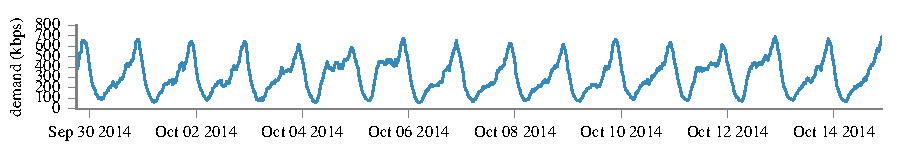
\includegraphics[width=\linewidth, 
height=12mm]{figures/mean_traffic_demand_per_subscriber_control.pdf}
  \caption{Control group with 105 Mbps service plan}
  \label{fig:traffic-load-control}
\end{subfigure}
%
\hspace{-1em}
%
\begin{subfigure}[b]{1\linewidth}
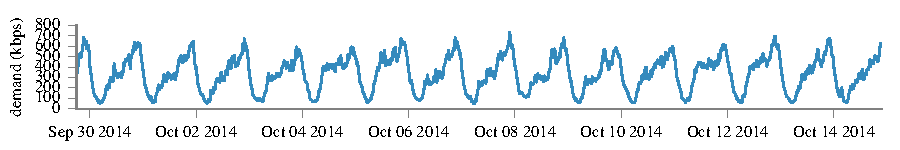
\includegraphics[width=\linewidth,, 
height=12mm]{figures/mean_traffic_demand_per_subscriber_treatment.pdf}
  \caption{Treatment group with 250 Mbps service upgrade}
  \label{fig:traffic-load-treatment}
\end{subfigure}
%\hfill
%
\end{minipage}
\caption{Mean traffic demand during the first two weeks of October\red{replace 
with bytes instead of kbps}}
\label{fig:traffic-load}
% created using docs/metadata-separated.log
\end{figure}


\begin{table*}[t]
\begin{tabular}{cccccccccc}
\hline
Dataset   & users & \multicolumn{2}{c}{Total Bytes} & \multicolumn{2}{c}{Avg. Traffic Demand} & \multicolumn{2}{c}{95\% Traffic Demand} & \multicolumn{2}{c}{Utilization} \\
          &       & up             & dw             & up                 & dw                 & up                 & dw                 & up             & dw             \\
control   & 4845  & 1.44e14        & 1.29e15        & 38.43              & 343.83             & 155.73             & 1769.65            & 0.14\%         & 1.65\%         \\
treatment & 1519  & 6.48e13        & 4.47e14        & 55.64              & 384.14             & 227.41             & 1944.01            & 0.21\%         & 1.81\%         \\ \hline
\end{tabular}
\caption{TODO: make it bytes instead of kbps. Equalize control and treatment 
using a multiplier to center = 1519/5845?
 Average traffic demand is the average data rate per subscriber 
 calculated by averaging the bytes transferred over the 15 minute time period. 
 The 95 percentile demand only averages the traffic data rate per subscriber 
for the top 95\% usage. Utilization (util.) is the ratio of 95\%ile traffic 
demand to the service tier capacity that the subscribers pay for: 105 Mbps. The 
utilization of observed in this data set is less than 2 \%}
\label{tab:data-stats}
\end{table*}

% \begin{table*}[ht]
% \small
% \begin{tabular}{ c | c | c | c | c | c | c | c | c | c }\hline
% \textbf{Dataset}      & \textbf{users} & \textbf{Bytes (up)}	
% & \textbf{Bytes (dw)} & \textbf{Average (up)}	& \textbf{Average 
% (dw)}	& \textbf{95\% (up)} & \textbf{95\% (dw)} & \textbf{Util. 
% (up)} & \textbf{Util. (dw)}\\\hline
% \control\footnote{unsanitized}		& & & & & & & & & \\
% \treatment\footnote{unsanitized}		& & & & & & & & & \\
% \control{}			& & & & & & & & & \\
% \treatment{}			& & & & & & & & & \\\hline
% \end{tabular}
% \caption{Data characteristics for datasets before and after sanitization. 
% Average traffic demand (kbps) is the average data rate per subscriber 
% calculated by averaging the bytes transferred over the 15 minute time period. 
% The 95 percentile demand only averages the traffic data rate per subscriber for 
% the top 95\% usage. Utilization (util.) is the ratio of 95\%ile traffic demand 
% to the service tier capacity that the subscribers pay for: 105 Mbps.}
% \label{tab:data-stats}
% \end{table*}


\paragraph{Data Characterization: }Our sanitized dataset consisted of 4,845 
subscribers in the \control{} group and 1,519 subscribers in the \treatment{}. 
The mean traffic usage per subscriber was \todo{XXX} bytes for the \control{} 
group and \todo{XXX} bytes for the \treatment{} every 15 minutes. We interpret 
the traffic transferred over uplink or downlink in 15 minutes in terms of the 
average traffic demand (data rate) by averaging it over the measurement period 
to effectively compare demand with the service capacity.

Figure \ref{fig:traffic-load} shows the average subscriber traffic demand 
(data rate) for both groups. The Service Level Agreement with Comcast was 105 
Mbps (upgraded to 250 Mbps) and is not shown in the figure due to the 
difference in scale. Table \ref{tab:data-stats} shows that the 95 percentile 
utilization, calculated as the ratio of the mean 95 
percentile traffic demand to the service capacity, is \todo{YYY} averaged 
over the \control{} group and \todo{YYY} for the treatment group. In 
comparison, the mean traffic demand is extremely similar, \todo{ZZZ} for the 
\control{} group and \todo{ZZZ} for the \treatment{}.